\section{Electricity and magnetism}
\subsection{Simple magnetism and magnetic fields}

// majorly to do

\begin{point}
Describe the forces between magnetic poles and between magnets and magnetic materials, including 
the use of the terms north pole (N pole), south pole (S pole), attraction and repulsion, magnetised and 
unmagnetised
\end{point}

\begin{point}
	Describe induced magnetism
\end{point}

\begin{point}
	State the difference between magnetic and non-magnetic materials
\end{point}

\subsection{Electrical quantities}
\subsubsection{Electrical charge}

\begin{subpoint}
State that there are positive and negative charges and that charge is measured in coulombs
\end{subpoint}

Matter is made of subatomic particles, two of which are \ul{\emph{protons}} and \ul{\emph{electrons}}.
These are positively and negatively charged, respectively. The magnitude of their charges are
measured in \ul{\emph{coulombs}} (C), the unit of \ul{\emph{charge}}.

Note that, though the particles have oppositely signed charge, the magnitudes of their charges are
equal, which is $1.6 \times 10^{-19}$ C.

\begin{subpoint}
State that unlike charges attract and like charges repel
\end{subpoint}

As in magnetism, only, here the the signs of the charges are to be the factors that cause attraction or
repulsion. Oppositely signed charges attract (positive and negative) and equally signed charges
repel.

\begin{subpoint}
Describe experiments to show electrostatic charging by friction
\end{subpoint}

As described before, charge is caused by the presence of protons and electrons. Protons are 
present in the nuclei of atoms, and are largely immobile. Electrons are present on the outskirts
of each atom and are very prone to movement.

In a \emph{electrically neutral} object, the number of protons equals the number of electrons,
their opposite charges cancelling out, producing a net charge of zero. However, for an object
with a \emph{lack of electrons} such that there are more protons than electrons, the object will
have a net charge that is positive. An object with an \emph{excess of electrons} has an overall
negative charge.

There are generally two types of materials in terms of how freely electrons can traverse them.
These are \ul{\emph{conductors}} and \ul{\emph{insulators}}. In an electrical conductor, the 
electrons can easily move through the object, but for electrical insulators, the electrons are
bound very strongly to their nuclei, making it difficult for them to move through the solid.

\smallskip
We can bring about a lack or excess of electrons by applying friction amongst two electrical
insulators. Rubbing two insulators together causes electrons to move from one to the other. This
causes an excess of electrons in one object, and a lack of electrons in the other. As a result,
the objects become oppositely charged. Bringing these close together, we find that they are 
attracted to each other.

This is only possible in insulators, as, if an electrostatic charge was brought into a metal and
it contacted any object, the excess electrons would flow out of it or electrons would be conducted
into it from the surroundings to undo the charge.

\begin{subpoint}
Explain that charging of solids by friction involves only a transfer of negative charge (electrons)
\end{subpoint}

\begin{subpoint}
Describe an electric field as a region in which an electric charge experiences a force
\end{subpoint}

\begin{subpoint}
State that the direction of an electric field line at a point is the direction of the force on a positive charge at 
that point
\end{subpoint}

A charged object has an \ul{\emph{electric field}} around it. This is a region in space where a charge will
experience a force. The direction of an electric field at a point is identical to the direction
of the force experienced by a positive charge at that point. 

Since a positive charge is always repelled away from another positive charge and attracted to
negative charges, electrical field
lines always have an outward direction from positive charges and an inward direction from negative
charges.

\begin{subpoint}
Describe simple electric field patterns, including the direction of the field:
\begin{enumerate}[label=(\alph*)]
	\setlength\itemsep{0em}
	\item around a point charge
	\item around a charged conducting sphere
	\item between two oppositely charged parallel conducting plates (end effects will not be examined)
\end{enumerate}
\end{subpoint}

Observe Figures 7 and 8.

\begin{figure}
	\centering
	\begin{tikzpicture}[
			decoration={
				markings,
				mark=at position 0.5 with {\arrow{>}}
			}
		]
		\draw (0, 0) circle (0.2) node{$+$};
		\draw[postaction=decorate] (0.2, 0) -- (1, 0);
		\draw[postaction=decorate] (-0.2, 0) -- (-1, 0);
		\draw[postaction=decorate] (0, 0.2) -- (0, 1);
		\draw[postaction=decorate] (0, -0.2) -- (0, -1);
		\draw[postaction=decorate] (0.14, 0.14) -- (0.7, 0.7); % Top-right
		\draw[postaction=decorate] (-0.14, 0.14) -- (-0.7, 0.7); % Top-left
		\draw[postaction=decorate] (-0.14, -0.14) -- (-0.7, -0.7); % Bottom-left
		\draw[postaction=decorate] (0.14, -0.14) -- (0.7, -0.7); % Bottom-right
	\end{tikzpicture} \hspace{1cm}
	\begin{tikzpicture}[
			decoration={
				markings,
				mark=at position 0.5 with {\arrow{<}}
			}
		]
		\draw (0, 0) circle (0.2) node{$-$};
		\draw[postaction=decorate] (0.2, 0) -- (1, 0);
		\draw[postaction=decorate] (-0.2, 0) -- (-1, 0);
		\draw[postaction=decorate] (0, 0.2) -- (0, 1);
		\draw[postaction=decorate] (0, -0.2) -- (0, -1);
		\draw[postaction=decorate] (0.14, 0.14) -- (0.7, 0.7); % Top-right
		\draw[postaction=decorate] (-0.14, 0.14) -- (-0.7, 0.7); % Top-left
		\draw[postaction=decorate] (-0.14, -0.14) -- (-0.7, -0.7); % Bottom-left
		\draw[postaction=decorate] (0.14, -0.14) -- (0.7, -0.7); % Bottom-right
	\end{tikzpicture}
	\caption{Electric field around  point charges}
\end{figure}

\begin{figure}
	\centering
	\begin{tikzpicture}[
        decoration={
            markings,
            mark=at position 0.5 with {\arrow{>}}
        }
    ]
    % Draw the plates
    \draw[thick] (-2, 1) -- (2, 1) node[midway, above] {$+++++++++++$};
    \draw[thick] (-2, -1) -- (2, -1) node[midway, below] {$-----------$};

    % Electric field lines
    \foreach \x in {-1.8, -1.2, -0.6, 0, 0.6, 1.2, 1.8} {
        \draw[postaction=decorate] (\x, 1) -- (\x, -1);
    }
	\end{tikzpicture}
	\caption{Electric field between oppositely charged conducting plates}
\end{figure}

Electric fields around point charges and charged, conducing spheres are identical; directed
radially outward and radially inward for positive and negatively charged spheres respectively.

\begin{subpoint}
State examples of electrical conductors and insulators
\end{subpoint}

All metals are great electrical conductors, whereas non metals are all insulators. Copper and gold
are phenomenal conductors whereas poly(ethene) and wood are insulators.

\begin{subpoint}
Describe an experiment to distinguish between electrical conductors and insulators
\end{subpoint}

\begin{figure}
	\centering
	\begin{circuitikz}
		\draw (0, 0) to[battery1] (2, 0)
		to [rmeter, t=A] (3, 0)
		to [short] (4, 0)
		to [short] (4, -2)
		to [european resistor, l_=material to be tested] (0.25, -2) 
		to [short] (0, -2) 
		to [short] (0, 0);
	\end{circuitikz}
	\caption{Circuit to see conductivity of material}
\end{figure}

Observe Figure 9, the resistor here, is the material to be tested. The ammeter will show the
extent of current that can flow through it. That reading indicates the extent of conductive
characteristic the material shows.

\begin{subpoint}
Recall and use a simple electron model to explain the difference between electrical conductors and 
insulators
\end{subpoint}

\subsubsection{Electrical current}

\begin{subpoint}
Define electric current as the charge passing a point per unit time; recall and use the equation
$$ \textrm{(electric current)} = \frac{\textrm{(charge)}}{\textrm{(time)}} $$
$$ I = \frac{Q}{t} $$
\end{subpoint}

\begin{subpoint}
Describe electrical conduction in metals in terms of the movement of free electrons
\end{subpoint}

Something that conducts electricity has free electrons that can move through it.

\begin{subpoint}
Know that current is measured in amps (amperes) and that the amp is given by coulomb per second (C/s)
\end{subpoint}

An ampere of current is identical to one coulomb of charge flowing through a point every second.
The shortened form of ampere is (A).

\begin{subpoint}
Know the difference between direct current (d.c.) and alternating current (a.c.)
\end{subpoint}

Current whose direction changes is said to \ul{\emph{alternating}}, otherwise it is \ul{\emph{direct}}.
The direction of current depends on the sign, change in sign means change in direction of flow
of current.

\begin{subpoint}
State that conventional current is from positive to negative and that the flow of free electrons is from 
negative to positive
\end{subpoint}

Free electrons flow from negative to positive terminals, whereas \emph{\ul{conventional current}} is considered
to flow form positive to negative. This is a historical mistake.

\begin{subpoint}
Describe the use of ammeters (analogue and digital) with different ranges
\end{subpoint}

Ammeters measure the amount of current flowing through them. In a circuit, they must always be
connected in series to the branch of whose current is being measured. 

Given a range of possible values,
the ammeter to be chosen is selected depending on which has a greater maximum range, but the
least difference between the greatest maximum range and the greatest possible anticipated value.

\subsubsection{Electromotive force and potential difference}

\begin{subpoint}
Define e.m.f. (electromotive force) as the electrical work done by a source in moving a unit charge around a 
complete circuit; recall and use the equation

$$ \textrm{(e.m.f.)} = \frac{\textrm{(work done (by a source))}}{\textrm{(charge)}} $$
$$ E = \frac{W}{Q} $$
\end{subpoint}

\begin{subpoint}
Define p.d. (potential difference) as the work done by a unit charge passing through a component; recall 
and use the equation

$$ \textrm{(p.d.)} = \frac{\textrm{(work done (on component))}}{\textrm{(charge}} $$
$$ V = \frac{W}{Q} $$
\end{subpoint}

\begin{subpoint}
Know that e.m.f. and p.d. are measured in volts and that the volt is given by joule per coulomb (J/C)
\end{subpoint}

The symbol of the volt is (V).

\begin{subpoint}
Describe the use of voltmeters (analogue and digital) with different ranges
\end{subpoint}

Identical to Section 2.2.2.6, only here, the voltmeters must be connected parallel to the 
component whose voltage is being measured.

\begin{subpoint}
Calculate the total e.m.f. where several sources are arranged in series
\end{subpoint}

Given there are $n$ source, with electromotive forces of $E_1$, $E_2$, $E_3$, ... $E_n$,
their total electromotive force equals:

$$ E_1 + E_2 + E_3 + ... + E_n $$

\begin{subpoint}
State that the e.m.f of identical sources connected in parallel is equal to the e.m.f. of one of the sources
\end{subpoint}

\subsubsection{Resistance}
\begin{subpoint}
Recall and use the equation
$$ \textrm{(resistance)} = \frac{\textrm{(p.d.)}}{\textrm{(current)}} $$
$$ R = \frac{V}{I} $$
\end{subpoint}

The resistance of a component is the voltage required to push one unit of charge through the
component. It is measured in ohms, whose symbol is ($\Omega$).

\begin{subpoint}
Describe an experiment to determine resistance using a voltmeter and an ammeter and do the appropriate 
calculations
\end{subpoint}

\begin{figure}
	\centering
	\begin{circuitikz}
		% \draw (-2, 0) to [battery1] (2, 0)
		% 	to [ammeter] (2, -1) 
		% 	to [short] (1, -1) 
		% 	to [short] (1, -2)
		% 	to [voltmeter] (-1, -2)
		% 	to [short] (-1, -1)
		% 	to [short] (-2, -1)
		% 	to [short] (-2, 0);
		% \draw (1, -1) [european resistor] (-1, -1);
			% Battery
			\draw
			(0,0) to[short] (0,2) % One-cell battery
			
			% European Resistor
			to[european resistor, l_=$R$] (3,2) % Resistor in series
			
			% Ammeter
			to[rmeter, t=A, l=$I$] (3,0) % Ammeter in series
			
			% Connect back to battery
			to [battery1] (0,0);
			
			% Voltmeter across the resistor
			\draw
			(0, 2) [short] to (0, 3)
			to[rmeter, l^=$V$, t=V] (3,3)
			to[short] (3, 2);
	\end{circuitikz}
	\caption{Experiment to determine resistance of component}
\end{figure}

Observe Figure 10. Here, the component whose resistance, $R$ is being determined is in series
to an ammeter and a source, and parallel to a voltmeter. The ammeter gives reading $I$ and the
voltmeter gives reading $V$. Hence,
$$ R = V/I $$

\begin{subpoint}
Recall and use, for a wire, the direct proportionality between resistance and length, and the inverse 
proportionality between resistance and cross-sectional area
\end{subpoint}

Consider the case of a conducting wire. Its resistance to current will depend on its physical
dimensions. That is, the longer the wire, the more resistant it will be, the thicker the wire
(the larger the cross section) the less resistant it will be. Symbolically

$$ R \propto L $$
$$ R \propto 1/A $$
where $L$ is the length of the wire and $A$ is its cross sectional area.

\begin{subpoint}
State Ohm’s law, including reference to constant temperature
\end{subpoint}

Ohm's law states that current across a resistor, at a constant temperature, will vary directly
with the voltage applied across it. Mathematically,

\begin{align*}
	V &\propto I \\ 
	V &= IR
\end{align*}
Here, the constant of proportionality is resistance.

\begin{subpoint}
Sketch and explain the current–voltage graphs for a resistor of constant resistance, a filament lamp and a 
diode
\end{subpoint}

\begin{figure}
	\centering
	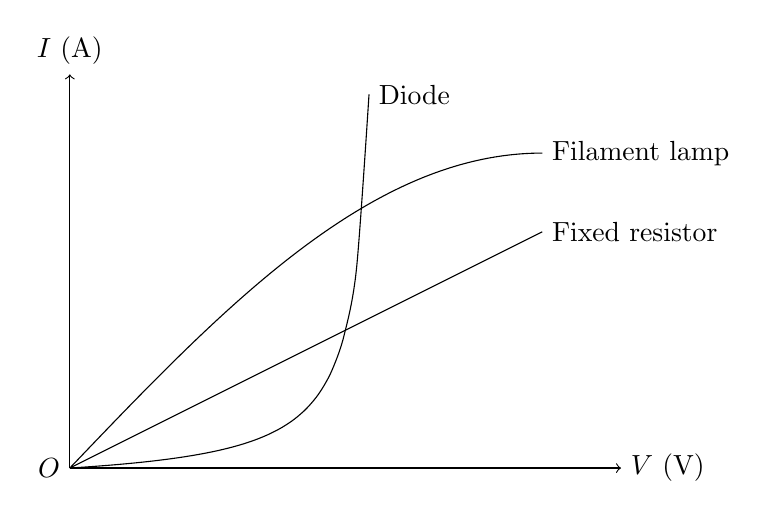
\begin{tikzpicture}
		\draw[->] (0, 0) -- (7, 0) node[right]{$V$ (V)};
		\draw [->] (0, 0) -- (0, 5) node[above]{$I$ (A)};
		\node (0, 0) [left]{$O$};

		\draw (0, 0) -- (6, 3) node[right]{Fixed resistor};
		\draw (0, 0) sin (6, 4) node[right]{Filament lamp};

		\draw[domain=0:3.8,smooth,variable=\x] 
			plot ({\x}, {-1/(\x-4) - 0.25}) 
			node[right] {Diode};
	\end{tikzpicture}
	\caption{Current-voltage graphs for constant resistance and a filament lamp}
\end{figure}

Observe Figure 11. A \ul{\emph{diode}} allows flow of infinite voltage once a sufficient voltage has been 
applied. 

For a \ul{\emph{filament lamp}}, the filament heats up as voltage across it is increased. As a result of this
increase in temperature, resistance across it also increases, inhibiting increase in voltage.

The \ul{\emph{fixed resistor}} shows the ohmic property of $V \propto I$.

\begin{point}
Describe the effect of temperature increase on the resistance of a resistor, such as the filament in a 
filament lamp
\end{point}

Increase in temperature increases resistance as the vibrating particles of the wire inhibit
smooth flow of charge.

\subsection{Electric circuits}
\subsubsection{Circuit diagrams and circuit components}

\begin{subpoint}
Draw and interpret circuit diagrams with cells, batteries, power supplies, generators, oscilloscopes, 
potential dividers, switches, resistors (fixed and variable), heaters, thermistors (NTC only), light-dependent 
resistors (LDRs), lamps, motors, ammeters, voltmeters, magnetising coils, transformers, fuses, relays, 
diodes and light-emitting diodes (LEDs), and know how these components behave in the circuit
\end{subpoint}

Refer to the syllabus for these symbols.

\subsubsection{Series and parallel circuits}
\begin{subpoint}
Recall and use in calculations, the fact that:
\begin{enumerate}[label=(\alph*)]
	\setlength\itemsep{0em}
	\item the current at every point in a series circuit is the same
	\item the sum of the currents entering a junction in a parallel circuit is equal to the sum of the currents that 
		leave the junction
	\item the total p.d. across the components in a series circuit is equal to the sum of the individual p.d.s across 
		each component
	\item the p.d. across an arrangement of parallel resistances is the same as the p.d. across one branch in the 
		arrangement of the parallel resistances
\end{enumerate}
\end{subpoint}

\begin{subpoint}
Calculate the combined resistance of two or more resistors in series
\end{subpoint}

For $n$ resistors that are in series, the sum of their resistances is
$$ R_1 + R_2 + R_3 + ... + R_n $$

\begin{subpoint}
Calculate the combined resistance of two resistors in parallel
\end{subpoint}

For $n$ resistors in parallel, the sum of their resistances is
$$ \left(R_1^{-1} + R_2^{-1} + ... R_n^{-1}\right)^{-1} $$

\subsubsection{Action and use of circuit components}
\begin{subpoint}
Describe the action of negative temperature coefficient (NTC) thermistors and light-dependent resistors 
and explain their use as input sensors
\end{subpoint}

\begin{figure}
\centering
\begin{circuitikz}
	\draw (0, 0) to [thermistor] (2, 0);
	\draw (0, 2) to [european light dependent resistor] (2, 2);
\end{circuitikz}
\caption{Light dependent resistor and thermistor}
\end{figure}

Observe Figure 12, which show the circuit symbols for a \ul{\emph{light dependent resistor}} and
a \ul{\emph{thermistor}} (the light dependent resistor should not have a circle around it, refer
to the syllabus).

A thermistor's resistance \emph{increases as heat decreases} and vice versa. An LDR's resistance
\emph{increases as light intensity decreases} and vice versa. \ul{With increase in \emph{input}
intensity, resistance decreases}.

\begin{subpoint}
Describe the action of a variable potential divider
\end{subpoint}

\begin{figure}
	\centering
	\begin{circuitikz}
		\draw (-3, 0) to [battery, l^={$V$}] (3, 0)
			to [short] (3, -1)
			to [european resistor, l^={$R_f$}] (0, -1)
			to [tgeneric, l^={$R_v$}] (-3, -1)
			to [short] (-3, 0)
			;

		\draw (-3, -1) to [short, -*] (-3, -3);
		\draw (0, -1) to [short, -*] (0, -3);

		\draw (-1.5, -3) node{$V_\textrm{out}$};
	\end{circuitikz}
	\caption{A potential divider circuit}
\end{figure}

A \ul{\emph{potential divider}} divides the e.m.f. of a source into two, using the principle of series 
circuits where voltages are divided amongst resistors according to their resistances. Figure 13
shows such a circuit.

Here, the total resistance across the circuit is $\sum{R} = R_v + R_f$, where $R_v$ can be changed as it
is that of a variable resistor. Since $R_v$ can change, it can take up more or less of a fraction
of total resistance. The e.m.f. provided by the source, $V$ does not change, but the voltage,
$ V_\textrm{out}$ across the variable resistor changes when $R_v$ changes. Here,

$$ V_\textrm{out} = \frac{R_v}{\sum{R}} $$

\begin{subpoint}
Recall and use the equation for two resistors used as a potential divider
$$ \frac{R_1}{R_2} = \frac{V_1}{V_2} $$
\end{subpoint}

In a series circuit, the ratio of voltage across two resistors equals the ratio of their
resistances.

\subsection{Practical electricity}
\subsubsection{Uses of electricity}

\begin{subpoint}
State common uses of electricity, including heating, lighting, battery charging and powering motors and 
electronic systems
\end{subpoint}

\begin{subpoint}
State the advantages of connecting lamps in parallel in a lighting circuit
\end{subpoint}

Each lamp lights brighter as all of them are exposed to the same voltage. If one lamp goes out
of order, the others are unaffected.

\begin{subpoint}
Recall and use the equation

$$ \textrm{(power)} = \textrm{(voltage)} \times \textrm{(current)} $$
$$ P = VI $$
\end{subpoint}

The power expended by a component equals the product of the current flowing through it and the
voltage across it.

\begin{subpoint}
Recall and use the equation

$$ \textrm{(energy)} = \textrm{(current) $\times$ (voltage) $\times$ (time)} $$
$$ E = IVt $$
\end{subpoint}

The product of power and time equals the energy expended over that time period.

\begin{subpoint}
Define the kilowatt-hour (kWh) and calculate the cost of using electrical appliances where the energy unit 
is the kWh
\end{subpoint}

The kilowatt-hour is a unit of energy equivalent to the energy expended when one kilowatt of power
is produced in an hour.

\subsubsection{Electrical safety}
\begin{subpoint}
State the hazards of:
\begin{enumerate}[label=(\alph*)]
	\setlength\itemsep{0em}
	\item damaged insulation
	\item overheating cables
	\item damp conditions
	\item excess current from overloading of plugs, extension leads, single and multiple sockets
\end{enumerate}
when using a mains supply
\end{subpoint}

Damaged insulation will electrify metal parts of a device, such that when touched a current will
flow through the body of he who touched it down to earth.

Overheating cables will melt.

Water conducts electricity

Too many plugs is bad because too much voltage being pulled to each appliance will overload
and overheat the wire of the multiplug.

\begin{subpoint}
Explain the use and operation of trip switches and fuses and choose appropriate fuse ratings and trip switch 
settings
\end{subpoint}

The function of \emph{trip switches} and \emph{fuses} is to \emph{break the circuit}
when too much current flows through it. 

\ul{\emph{Fuses}} are lengths of thin wire, which will conduct 
current of a certain magnitude, but beyond a certain magnitude these fuses will melt and break
the circuit. The maximum current a fuse will tolerate is called its \ul{\emph{rating}}. The
fuse must hence be replaced each time it melts, feasible as the fuses are cheap.

\ul{\emph{Trip switches}} are mechanisms which disconnect a circuit when a current of certain
magnitude flows through them. These are also called circuit breakers, and these do not need
to be replaced after each disconnection. They are expensive, contrastingly to fuses.

\begin{subpoint}
Explain what happens when a live wire touches a metal case that is earthed
\end{subpoint}

Current flows through the metal casing, through the least resistance path, down to earth.

\begin{subpoint}
Explain why the outer casing of an electrical appliance must be either non-conducting (double-insulated) or 
earthed
\end{subpoint}

Non-conducting casings will never pass current onto user's body. Metal casings must be connected
to earth, when the casing is electrified, the earth connection is always less resistance than
the user's body, which causes current to flow down into earth, preventing an electric shock.

\begin{subpoint}
Know that a mains circuit consists of a live wire (line wire), a neutral wire and an earth wire and explain 
why a switch must be connected into the live wire for the circuit to be switched off safely
\end{subpoint}

The live wire is what carries the alternating current, and the neutral wire is what allows the
current to alternate, how exactly is out of the syllabus' scope. The earth wire connects to earth.

Since the live wire carries current, switching it on or off switches the appliance on or off.

\begin{subpoint}
Explain why fuses and circuit breakers are connected into the live wire
\end{subpoint}

If large magnitude of current flows as a result of broken insulation or metal casing or whatever,
they will flow through the live wire. As a result, circuit breaking mechanisms are connected
to the current-carrying live wire.
